\chapter{基于BLE Mesh的智能家居平台功能设计}

\section{架构设计}
本项目主要分为三个部分:BLE Mesh模块端,网关端及移动端,如图~\ref{fig:arch}。

BLE Mesh模块端主要实现传感器、继电器、灯泡等设备的接入,并且模块间可自动建立BLE协议下的Mesh网络,使得用户即使不使用网关也能用移动端软件连接至Mesh网络控制所有模块。

网关端主要实现设备层与管理应用层的连接。采用插件化的方案,使得有能力的爱好者或其他智能设备厂商,可以自己根据本项目简单的API来制作插件接入本平台;也便于接入到其他的管理平台,例如Apple HomeKit、Google Home等,让用户不需要下载其他程序就能管理网关下的所有设备。

移动端主要实现控制Mesh网络或网关下的设备、添加自动化的功能。
\begin{figure}[H]
    \centering
    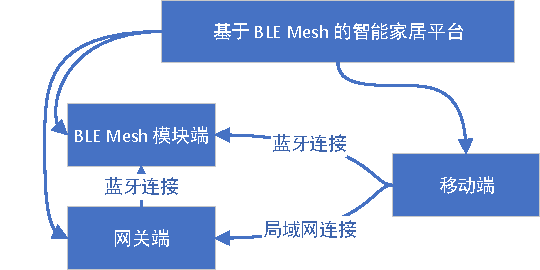
\includegraphics{arch.pdf}
    \caption{基于BLE Mesh的智能家居平台基本架构图}
    \label{fig:arch}
\end{figure}

\section{BLE Mesh模块端}
内容

\section{网关端}
内容

\section{移动端}
内容
